\documentclass[border=4pt]{standalone}
\usepackage[T1]{fontenc}
\usepackage{lmodern}
\usepackage{amsmath,amssymb}
\usepackage{tikz}
\usetikzlibrary{positioning,calc}
\usepackage{pgfplots}
\pgfplotsset{compat=1.18}

\definecolor{myblue}  {RGB}{55, 119, 189}
\definecolor{myred}   {RGB}{210,  70,  70}
\definecolor{mygreen} {RGB}{ 50, 155,  70}
\definecolor{myorange}{RGB}{230, 130,  40}
\definecolor{mygray}  {RGB}{130, 130, 130}

\begin{document}
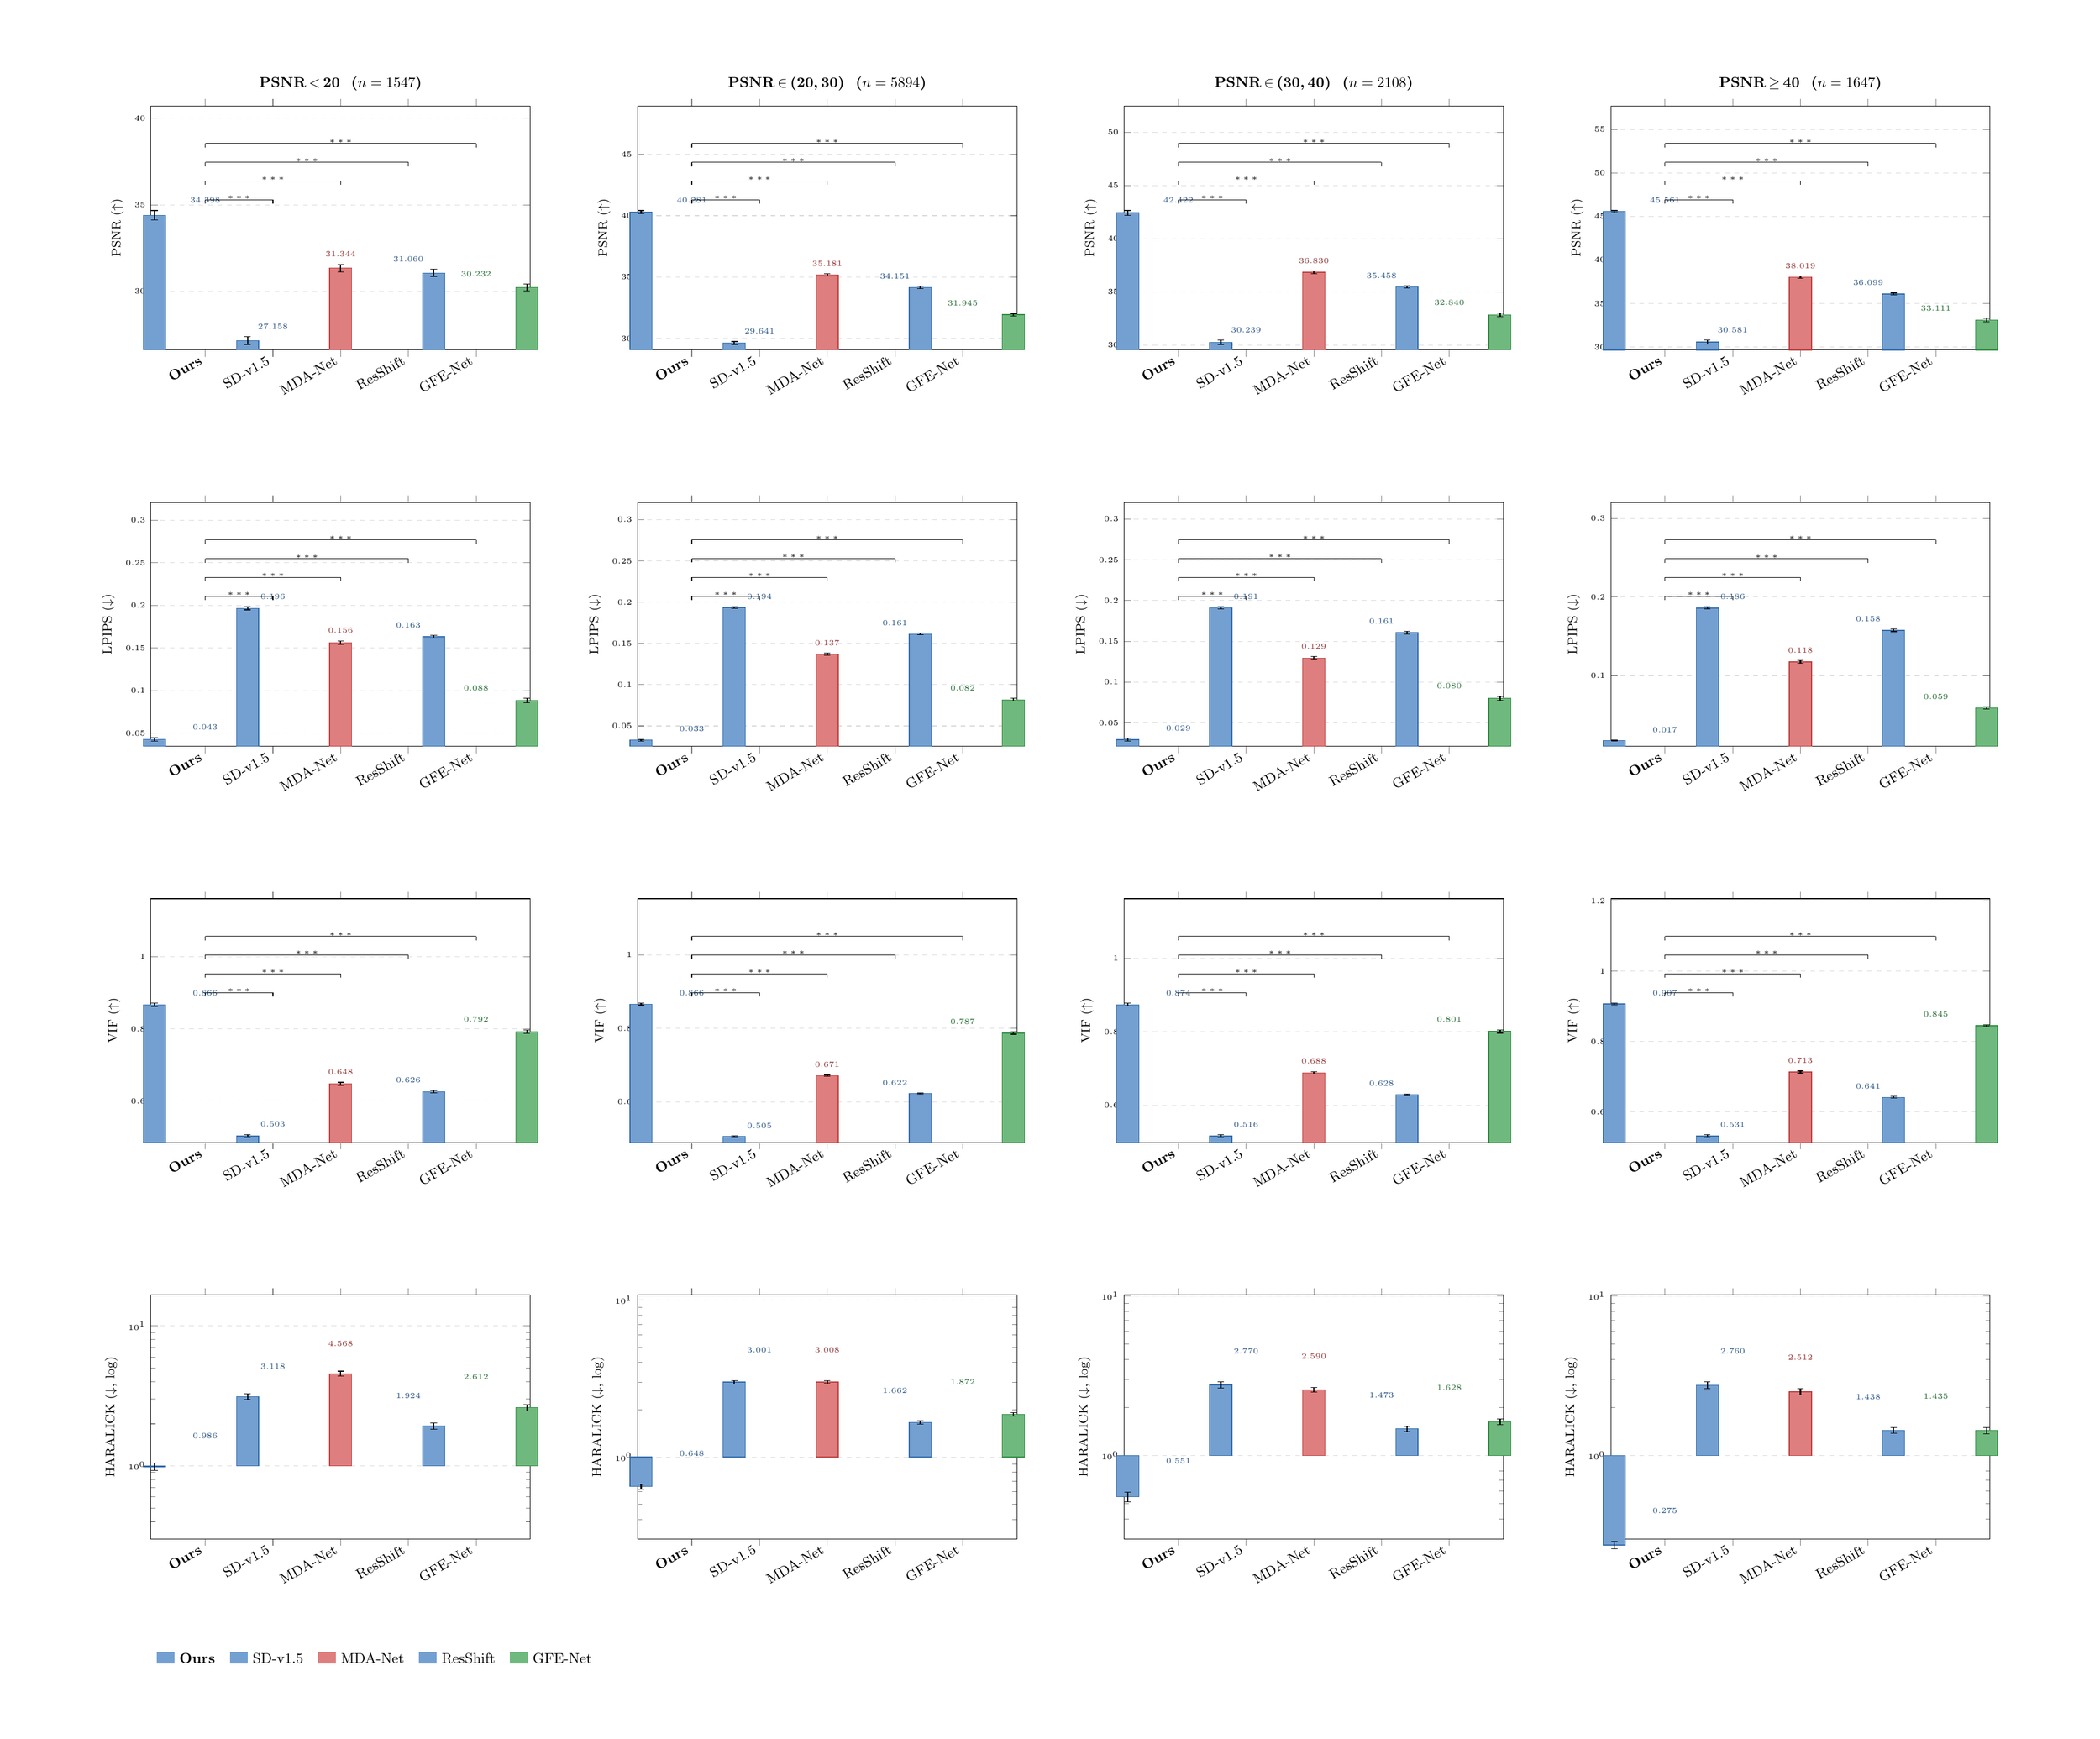
\begin{tikzpicture}[font=\small]
\useasboundingbox (-3.0cm,2.0cm) rectangle (42.9cm,-35.9cm);

% ── PSNR | PSNR<20 ──────────────────────────────────
\begin{axis}[
  name=ax00,
  at={(0.00cm,0.00cm)},
  anchor=north west,
  width=10.0cm,
  height=7.0cm,
  ybar,
  bar width=14pt,
  xtick={1,...,5},
  xticklabels={{\textbf{Ours}},{SD-v1.5},{MDA-Net},{ResShift},{GFE-Net}},
  xticklabel style={rotate=30, anchor=east, font=\small},
  ymin=26.6185,
  ymax=40.7139,
  xmin=0.2,
  xmax=5.8,
  ylabel={PSNR ($\uparrow$)},
  ylabel style={font=\footnotesize},
  ymajorgrids=true,
  grid style={dashed, gray!30},
  tick style={thin},
  every tick label/.style={font=\footnotesize},
  clip=false,
  scaled y ticks=false,
  y tick label style={font=\tiny, /pgf/number format/fixed, /pgf/number format/precision=3},
  title={PSNR\,$<$\,20\ \ ($n=1547$)},
  title style={font=\small\bfseries, align=center},
]

\addplot[
  ybar, fill=myblue!70, draw=myblue!90!black, line width=0.5pt,
  error bars/.cd, y dir=both, y explicit,
  error bar style={line width=0.8pt, black},
] coordinates {(1,34.3978) +- (0.2767,0.2752)};
\addplot[
  ybar, fill=myblue!70, draw=myblue!90!black, line width=0.5pt,
  error bars/.cd, y dir=both, y explicit,
  error bar style={line width=0.8pt, black},
] coordinates {(2,27.1577) +- (0.2294,0.2283)};
\addplot[
  ybar, fill=myred!70, draw=myred!90!black, line width=0.5pt,
  error bars/.cd, y dir=both, y explicit,
  error bar style={line width=0.8pt, black},
] coordinates {(3,31.3439) +- (0.2117,0.2158)};
\addplot[
  ybar, fill=myblue!70, draw=myblue!90!black, line width=0.5pt,
  error bars/.cd, y dir=both, y explicit,
  error bar style={line width=0.8pt, black},
] coordinates {(4,31.0604) +- (0.2203,0.2129)};
\addplot[
  ybar, fill=mygreen!70, draw=mygreen!90!black, line width=0.5pt,
  error bars/.cd, y dir=both, y explicit,
  error bar style={line width=0.8pt, black},
] coordinates {(5,30.2316) +- (0.1947,0.1866)};

\node[above, font=\tiny, inner sep=0pt, text=myblue!70!black] at (axis cs:1,35.0959) {34.398};
\node[above, font=\tiny, inner sep=0pt, text=myblue!70!black] at (axis cs:2,27.8089) {27.158};
\node[above, font=\tiny, inner sep=0pt, text=myred!70!black] at (axis cs:3,31.9826) {31.344};
\node[above, font=\tiny, inner sep=0pt, text=myblue!70!black] at (axis cs:4,31.6962) {31.060};
\node[above, font=\tiny, inner sep=0pt, text=mygreen!70!black] at (axis cs:5,30.8411) {30.232};
\draw[thin] (axis cs:1,35.2926) -- (axis cs:2,35.2926);
\draw[thin] (axis cs:1,35.2926) -- (axis cs:1,35.0602);
\draw[thin] (axis cs:2,35.2926) -- (axis cs:2,35.0602);
\node[above, font=\tiny, inner sep=0pt] at (axis cs:1.50,35.2926) {$***$};
\draw[thin] (axis cs:1,36.3768) -- (axis cs:3,36.3768);
\draw[thin] (axis cs:1,36.3768) -- (axis cs:1,36.1445);
\draw[thin] (axis cs:3,36.3768) -- (axis cs:3,36.1445);
\node[above, font=\tiny, inner sep=0pt] at (axis cs:2.00,36.3768) {$***$};
\draw[thin] (axis cs:1,37.4611) -- (axis cs:4,37.4611);
\draw[thin] (axis cs:1,37.4611) -- (axis cs:1,37.2288);
\draw[thin] (axis cs:4,37.4611) -- (axis cs:4,37.2288);
\node[above, font=\tiny, inner sep=0pt] at (axis cs:2.50,37.4611) {$***$};
\draw[thin] (axis cs:1,38.5454) -- (axis cs:5,38.5454);
\draw[thin] (axis cs:1,38.5454) -- (axis cs:1,38.3130);
\draw[thin] (axis cs:5,38.5454) -- (axis cs:5,38.3130);
\node[above, font=\tiny, inner sep=0pt] at (axis cs:3.00,38.5454) {$***$};
\end{axis}

% ── PSNR | (20, 30) ──────────────────────────────────
\begin{axis}[
  name=ax01,
  at={(10.80cm,0.00cm)},
  anchor=north west,
  width=10.0cm,
  height=7.0cm,
  ybar,
  bar width=14pt,
  xtick={1,...,5},
  xticklabels={{\textbf{Ours}},{SD-v1.5},{MDA-Net},{ResShift},{GFE-Net}},
  xticklabel style={rotate=30, anchor=east, font=\small},
  ymin=29.0735,
  ymax=48.9281,
  xmin=0.2,
  xmax=5.8,
  ylabel={PSNR ($\uparrow$)},
  ylabel style={font=\footnotesize},
  ymajorgrids=true,
  grid style={dashed, gray!30},
  tick style={thin},
  every tick label/.style={font=\footnotesize},
  clip=false,
  scaled y ticks=false,
  y tick label style={font=\tiny, /pgf/number format/fixed, /pgf/number format/precision=3},
  title={PSNR\,$\in$\,(20,\,30)\ \ ($n=5894$)},
  title style={font=\small\bfseries, align=center},
]

\addplot[
  ybar, fill=myblue!70, draw=myblue!90!black, line width=0.5pt,
  error bars/.cd, y dir=both, y explicit,
  error bar style={line width=0.8pt, black},
] coordinates {(1,40.2814) +- (0.1443,0.1376)};
\addplot[
  ybar, fill=myblue!70, draw=myblue!90!black, line width=0.5pt,
  error bars/.cd, y dir=both, y explicit,
  error bar style={line width=0.8pt, black},
] coordinates {(2,29.6414) +- (0.1315,0.1225)};
\addplot[
  ybar, fill=myred!70, draw=myred!90!black, line width=0.5pt,
  error bars/.cd, y dir=both, y explicit,
  error bar style={line width=0.8pt, black},
] coordinates {(3,35.1814) +- (0.1001,0.0916)};
\addplot[
  ybar, fill=myblue!70, draw=myblue!90!black, line width=0.5pt,
  error bars/.cd, y dir=both, y explicit,
  error bar style={line width=0.8pt, black},
] coordinates {(4,34.1509) +- (0.0955,0.0878)};
\addplot[
  ybar, fill=mygreen!70, draw=mygreen!90!black, line width=0.5pt,
  error bars/.cd, y dir=both, y explicit,
  error bar style={line width=0.8pt, black},
] coordinates {(5,31.9448) +- (0.0942,0.0973)};

\node[above, font=\tiny, inner sep=0pt, text=myblue!70!black] at (axis cs:1,41.0146) {40.281};
\node[above, font=\tiny, inner sep=0pt, text=myblue!70!black] at (axis cs:2,30.3595) {29.641};
\node[above, font=\tiny, inner sep=0pt, text=myred!70!black] at (axis cs:3,35.8686) {35.181};
\node[above, font=\tiny, inner sep=0pt, text=myblue!70!black] at (axis cs:4,34.8343) {34.151};
\node[above, font=\tiny, inner sep=0pt, text=mygreen!70!black] at (axis cs:5,32.6377) {31.945};
\draw[thin] (axis cs:1,41.2917) -- (axis cs:2,41.2917);
\draw[thin] (axis cs:1,41.2917) -- (axis cs:1,40.9645);
\draw[thin] (axis cs:2,41.2917) -- (axis cs:2,40.9645);
\node[above, font=\tiny, inner sep=0pt] at (axis cs:1.50,41.2917) {$***$};
\draw[thin] (axis cs:1,42.8190) -- (axis cs:3,42.8190);
\draw[thin] (axis cs:1,42.8190) -- (axis cs:1,42.4917);
\draw[thin] (axis cs:3,42.8190) -- (axis cs:3,42.4917);
\node[above, font=\tiny, inner sep=0pt] at (axis cs:2.00,42.8190) {$***$};
\draw[thin] (axis cs:1,44.3463) -- (axis cs:4,44.3463);
\draw[thin] (axis cs:1,44.3463) -- (axis cs:1,44.0190);
\draw[thin] (axis cs:4,44.3463) -- (axis cs:4,44.0190);
\node[above, font=\tiny, inner sep=0pt] at (axis cs:2.50,44.3463) {$***$};
\draw[thin] (axis cs:1,45.8736) -- (axis cs:5,45.8736);
\draw[thin] (axis cs:1,45.8736) -- (axis cs:1,45.5463);
\draw[thin] (axis cs:5,45.8736) -- (axis cs:5,45.5463);
\node[above, font=\tiny, inner sep=0pt] at (axis cs:3.00,45.8736) {$***$};
\end{axis}

% ── PSNR | (30, 40) ──────────────────────────────────
\begin{axis}[
  name=ax02,
  at={(21.60cm,0.00cm)},
  anchor=north west,
  width=10.0cm,
  height=7.0cm,
  ybar,
  bar width=14pt,
  xtick={1,...,5},
  xticklabels={{\textbf{Ours}},{SD-v1.5},{MDA-Net},{ResShift},{GFE-Net}},
  xticklabel style={rotate=30, anchor=east, font=\small},
  ymin=29.5316,
  ymax=52.4743,
  xmin=0.2,
  xmax=5.8,
  ylabel={PSNR ($\uparrow$)},
  ylabel style={font=\footnotesize},
  ymajorgrids=true,
  grid style={dashed, gray!30},
  tick style={thin},
  every tick label/.style={font=\footnotesize},
  clip=false,
  scaled y ticks=false,
  y tick label style={font=\tiny, /pgf/number format/fixed, /pgf/number format/precision=3},
  title={PSNR\,$\in$\,(30,\,40)\ \ ($n=2108$)},
  title style={font=\small\bfseries, align=center},
]

\addplot[
  ybar, fill=myblue!70, draw=myblue!90!black, line width=0.5pt,
  error bars/.cd, y dir=both, y explicit,
  error bar style={line width=0.8pt, black},
] coordinates {(1,42.4223) +- (0.2220,0.2194)};
\addplot[
  ybar, fill=myblue!70, draw=myblue!90!black, line width=0.5pt,
  error bars/.cd, y dir=both, y explicit,
  error bar style={line width=0.8pt, black},
] coordinates {(2,30.2391) +- (0.2033,0.2074)};
\addplot[
  ybar, fill=myred!70, draw=myred!90!black, line width=0.5pt,
  error bars/.cd, y dir=both, y explicit,
  error bar style={line width=0.8pt, black},
] coordinates {(3,36.8301) +- (0.1352,0.1363)};
\addplot[
  ybar, fill=myblue!70, draw=myblue!90!black, line width=0.5pt,
  error bars/.cd, y dir=both, y explicit,
  error bar style={line width=0.8pt, black},
] coordinates {(4,35.4577) +- (0.1141,0.1195)};
\addplot[
  ybar, fill=mygreen!70, draw=mygreen!90!black, line width=0.5pt,
  error bars/.cd, y dir=both, y explicit,
  error bar style={line width=0.8pt, black},
] coordinates {(5,32.8405) +- (0.1662,0.1622)};

\node[above, font=\tiny, inner sep=0pt, text=myblue!70!black] at (axis cs:1,43.3300) {42.422};
\node[above, font=\tiny, inner sep=0pt, text=myblue!70!black] at (axis cs:2,31.1348) {30.239};
\node[above, font=\tiny, inner sep=0pt, text=myred!70!black] at (axis cs:3,37.6547) {36.830};
\node[above, font=\tiny, inner sep=0pt, text=myblue!70!black] at (axis cs:4,36.2655) {35.458};
\node[above, font=\tiny, inner sep=0pt, text=mygreen!70!black] at (axis cs:5,33.6910) {32.840};
\draw[thin] (axis cs:1,43.6502) -- (axis cs:2,43.6502);
\draw[thin] (axis cs:1,43.6502) -- (axis cs:1,43.2720);
\draw[thin] (axis cs:2,43.6502) -- (axis cs:2,43.2720);
\node[above, font=\tiny, inner sep=0pt] at (axis cs:1.50,43.6502) {$***$};
\draw[thin] (axis cs:1,45.4150) -- (axis cs:3,45.4150);
\draw[thin] (axis cs:1,45.4150) -- (axis cs:1,45.0368);
\draw[thin] (axis cs:3,45.4150) -- (axis cs:3,45.0368);
\node[above, font=\tiny, inner sep=0pt] at (axis cs:2.00,45.4150) {$***$};
\draw[thin] (axis cs:1,47.1798) -- (axis cs:4,47.1798);
\draw[thin] (axis cs:1,47.1798) -- (axis cs:1,46.8016);
\draw[thin] (axis cs:4,47.1798) -- (axis cs:4,46.8016);
\node[above, font=\tiny, inner sep=0pt] at (axis cs:2.50,47.1798) {$***$};
\draw[thin] (axis cs:1,48.9446) -- (axis cs:5,48.9446);
\draw[thin] (axis cs:1,48.9446) -- (axis cs:1,48.5665);
\draw[thin] (axis cs:5,48.9446) -- (axis cs:5,48.5665);
\node[above, font=\tiny, inner sep=0pt] at (axis cs:3.00,48.9446) {$***$};
\end{axis}

% ── PSNR | (40, 40+) ──────────────────────────────────
\begin{axis}[
  name=ax03,
  at={(32.40cm,0.00cm)},
  anchor=north west,
  width=10.0cm,
  height=7.0cm,
  ybar,
  bar width=14pt,
  xtick={1,...,5},
  xticklabels={{\textbf{Ours}},{SD-v1.5},{MDA-Net},{ResShift},{GFE-Net}},
  xticklabel style={rotate=30, anchor=east, font=\small},
  ymin=29.6760,
  ymax=57.6796,
  xmin=0.2,
  xmax=5.8,
  ylabel={PSNR ($\uparrow$)},
  ylabel style={font=\footnotesize},
  ymajorgrids=true,
  grid style={dashed, gray!30},
  tick style={thin},
  every tick label/.style={font=\footnotesize},
  clip=false,
  scaled y ticks=false,
  y tick label style={font=\tiny, /pgf/number format/fixed, /pgf/number format/precision=3},
  title={PSNR\,$\geq$\,40\ \ ($n=1647$)},
  title style={font=\small\bfseries, align=center},
]

\addplot[
  ybar, fill=myblue!70, draw=myblue!90!black, line width=0.5pt,
  error bars/.cd, y dir=both, y explicit,
  error bar style={line width=0.8pt, black},
] coordinates {(1,45.5607) +- (0.1439,0.1174)};
\addplot[
  ybar, fill=myblue!70, draw=myblue!90!black, line width=0.5pt,
  error bars/.cd, y dir=both, y explicit,
  error bar style={line width=0.8pt, black},
] coordinates {(2,30.5805) +- (0.2890,0.2224)};
\addplot[
  ybar, fill=myred!70, draw=myred!90!black, line width=0.5pt,
  error bars/.cd, y dir=both, y explicit,
  error bar style={line width=0.8pt, black},
] coordinates {(3,38.0191) +- (0.1364,0.1264)};
\addplot[
  ybar, fill=myblue!70, draw=myblue!90!black, line width=0.5pt,
  error bars/.cd, y dir=both, y explicit,
  error bar style={line width=0.8pt, black},
] coordinates {(4,36.0989) +- (0.1266,0.1254)};
\addplot[
  ybar, fill=mygreen!70, draw=mygreen!90!black, line width=0.5pt,
  error bars/.cd, y dir=both, y explicit,
  error bar style={line width=0.8pt, black},
] coordinates {(5,33.1113) +- (0.1967,0.1906)};

\node[above, font=\tiny, inner sep=0pt, text=myblue!70!black] at (axis cs:1,46.5182) {45.561};
\node[above, font=\tiny, inner sep=0pt, text=myblue!70!black] at (axis cs:2,31.6430) {30.581};
\node[above, font=\tiny, inner sep=0pt, text=myred!70!black] at (axis cs:3,38.9856) {38.019};
\node[above, font=\tiny, inner sep=0pt, text=myblue!70!black] at (axis cs:4,37.0644) {36.099};
\node[above, font=\tiny, inner sep=0pt, text=mygreen!70!black] at (axis cs:5,34.1420) {33.111};
\draw[thin] (axis cs:1,46.9090) -- (axis cs:2,46.9090);
\draw[thin] (axis cs:1,46.9090) -- (axis cs:1,46.4474);
\draw[thin] (axis cs:2,46.9090) -- (axis cs:2,46.4474);
\node[above, font=\tiny, inner sep=0pt] at (axis cs:1.50,46.9090) {$***$};
\draw[thin] (axis cs:1,49.0632) -- (axis cs:3,49.0632);
\draw[thin] (axis cs:1,49.0632) -- (axis cs:1,48.6016);
\draw[thin] (axis cs:3,49.0632) -- (axis cs:3,48.6016);
\node[above, font=\tiny, inner sep=0pt] at (axis cs:2.00,49.0632) {$***$};
\draw[thin] (axis cs:1,51.2173) -- (axis cs:4,51.2173);
\draw[thin] (axis cs:1,51.2173) -- (axis cs:1,50.7557);
\draw[thin] (axis cs:4,51.2173) -- (axis cs:4,50.7557);
\node[above, font=\tiny, inner sep=0pt] at (axis cs:2.50,51.2173) {$***$};
\draw[thin] (axis cs:1,53.3714) -- (axis cs:5,53.3714);
\draw[thin] (axis cs:1,53.3714) -- (axis cs:1,52.9098);
\draw[thin] (axis cs:5,53.3714) -- (axis cs:5,52.9098);
\node[above, font=\tiny, inner sep=0pt] at (axis cs:3.00,53.3714) {$***$};
\end{axis}

% ── LPIPS | PSNR<20 ──────────────────────────────────
\begin{axis}[
  name=ax10,
  at={(0.00cm,-8.80cm)},
  anchor=north west,
  width=10.0cm,
  height=7.0cm,
  ybar,
  bar width=14pt,
  xtick={1,...,5},
  xticklabels={{\textbf{Ours}},{SD-v1.5},{MDA-Net},{ResShift},{GFE-Net}},
  xticklabel style={rotate=30, anchor=east, font=\small},
  ymin=0.0345,
  ymax=0.3208,
  xmin=0.2,
  xmax=5.8,
  ylabel={LPIPS ($\downarrow$)},
  ylabel style={font=\footnotesize},
  ymajorgrids=true,
  grid style={dashed, gray!30},
  tick style={thin},
  every tick label/.style={font=\footnotesize},
  clip=false,
  scaled y ticks=false,
  y tick label style={font=\tiny, /pgf/number format/fixed, /pgf/number format/precision=3},
]

\addplot[
  ybar, fill=myblue!70, draw=myblue!90!black, line width=0.5pt,
  error bars/.cd, y dir=both, y explicit,
  error bar style={line width=0.8pt, black},
] coordinates {(1,0.0427) +- (0.0019,0.0021)};
\addplot[
  ybar, fill=myblue!70, draw=myblue!90!black, line width=0.5pt,
  error bars/.cd, y dir=both, y explicit,
  error bar style={line width=0.8pt, black},
] coordinates {(2,0.1964) +- (0.0017,0.0017)};
\addplot[
  ybar, fill=myred!70, draw=myred!90!black, line width=0.5pt,
  error bars/.cd, y dir=both, y explicit,
  error bar style={line width=0.8pt, black},
] coordinates {(3,0.1562) +- (0.0024,0.0022)};
\addplot[
  ybar, fill=myblue!70, draw=myblue!90!black, line width=0.5pt,
  error bars/.cd, y dir=both, y explicit,
  error bar style={line width=0.8pt, black},
] coordinates {(4,0.1631) +- (0.0018,0.0018)};
\addplot[
  ybar, fill=mygreen!70, draw=mygreen!90!black, line width=0.5pt,
  error bars/.cd, y dir=both, y explicit,
  error bar style={line width=0.8pt, black},
] coordinates {(5,0.0882) +- (0.0026,0.0028)};

\node[above, font=\tiny, inner sep=0pt, text=myblue!70!black] at (axis cs:1,0.0534) {0.043};
\node[above, font=\tiny, inner sep=0pt, text=myblue!70!black] at (axis cs:2,0.2067) {0.196};
\node[above, font=\tiny, inner sep=0pt, text=myred!70!black] at (axis cs:3,0.1670) {0.156};
\node[above, font=\tiny, inner sep=0pt, text=myblue!70!black] at (axis cs:4,0.1735) {0.163};
\node[above, font=\tiny, inner sep=0pt, text=mygreen!70!black] at (axis cs:5,0.0996) {0.088};
\draw[thin] (axis cs:1,0.2107) -- (axis cs:2,0.2107);
\draw[thin] (axis cs:1,0.2107) -- (axis cs:1,0.2060);
\draw[thin] (axis cs:2,0.2107) -- (axis cs:2,0.2060);
\node[above, font=\tiny, inner sep=0pt] at (axis cs:1.50,0.2107) {$***$};
\draw[thin] (axis cs:1,0.2327) -- (axis cs:3,0.2327);
\draw[thin] (axis cs:1,0.2327) -- (axis cs:1,0.2280);
\draw[thin] (axis cs:3,0.2327) -- (axis cs:3,0.2280);
\node[above, font=\tiny, inner sep=0pt] at (axis cs:2.00,0.2327) {$***$};
\draw[thin] (axis cs:1,0.2547) -- (axis cs:4,0.2547);
\draw[thin] (axis cs:1,0.2547) -- (axis cs:1,0.2500);
\draw[thin] (axis cs:4,0.2547) -- (axis cs:4,0.2500);
\node[above, font=\tiny, inner sep=0pt] at (axis cs:2.50,0.2547) {$***$};
\draw[thin] (axis cs:1,0.2767) -- (axis cs:5,0.2767);
\draw[thin] (axis cs:1,0.2767) -- (axis cs:1,0.2720);
\draw[thin] (axis cs:5,0.2767) -- (axis cs:5,0.2720);
\node[above, font=\tiny, inner sep=0pt] at (axis cs:3.00,0.2767) {$***$};
\end{axis}

% ── LPIPS | (20, 30) ──────────────────────────────────
\begin{axis}[
  name=ax11,
  at={(10.80cm,-8.80cm)},
  anchor=north west,
  width=10.0cm,
  height=7.0cm,
  ybar,
  bar width=14pt,
  xtick={1,...,5},
  xticklabels={{\textbf{Ours}},{SD-v1.5},{MDA-Net},{ResShift},{GFE-Net}},
  xticklabel style={rotate=30, anchor=east, font=\small},
  ymin=0.0252,
  ymax=0.3211,
  xmin=0.2,
  xmax=5.8,
  ylabel={LPIPS ($\downarrow$)},
  ylabel style={font=\footnotesize},
  ymajorgrids=true,
  grid style={dashed, gray!30},
  tick style={thin},
  every tick label/.style={font=\footnotesize},
  clip=false,
  scaled y ticks=false,
  y tick label style={font=\tiny, /pgf/number format/fixed, /pgf/number format/precision=3},
]

\addplot[
  ybar, fill=myblue!70, draw=myblue!90!black, line width=0.5pt,
  error bars/.cd, y dir=both, y explicit,
  error bar style={line width=0.8pt, black},
] coordinates {(1,0.0328) +- (0.0011,0.0011)};
\addplot[
  ybar, fill=myblue!70, draw=myblue!90!black, line width=0.5pt,
  error bars/.cd, y dir=both, y explicit,
  error bar style={line width=0.8pt, black},
] coordinates {(2,0.1935) +- (0.0008,0.0008)};
\addplot[
  ybar, fill=myred!70, draw=myred!90!black, line width=0.5pt,
  error bars/.cd, y dir=both, y explicit,
  error bar style={line width=0.8pt, black},
] coordinates {(3,0.1370) +- (0.0013,0.0013)};
\addplot[
  ybar, fill=myblue!70, draw=myblue!90!black, line width=0.5pt,
  error bars/.cd, y dir=both, y explicit,
  error bar style={line width=0.8pt, black},
] coordinates {(4,0.1614) +- (0.0009,0.0010)};
\addplot[
  ybar, fill=mygreen!70, draw=mygreen!90!black, line width=0.5pt,
  error bars/.cd, y dir=both, y explicit,
  error bar style={line width=0.8pt, black},
] coordinates {(5,0.0817) +- (0.0016,0.0017)};

\node[above, font=\tiny, inner sep=0pt, text=myblue!70!black] at (axis cs:1,0.0428) {0.033};
\node[above, font=\tiny, inner sep=0pt, text=myblue!70!black] at (axis cs:2,0.2032) {0.194};
\node[above, font=\tiny, inner sep=0pt, text=myred!70!black] at (axis cs:3,0.1472) {0.137};
\node[above, font=\tiny, inner sep=0pt, text=myblue!70!black] at (axis cs:4,0.1713) {0.161};
\node[above, font=\tiny, inner sep=0pt, text=mygreen!70!black] at (axis cs:5,0.0923) {0.082};
\draw[thin] (axis cs:1,0.2073) -- (axis cs:2,0.2073);
\draw[thin] (axis cs:1,0.2073) -- (axis cs:1,0.2024);
\draw[thin] (axis cs:2,0.2073) -- (axis cs:2,0.2024);
\node[above, font=\tiny, inner sep=0pt] at (axis cs:1.50,0.2073) {$***$};
\draw[thin] (axis cs:1,0.2301) -- (axis cs:3,0.2301);
\draw[thin] (axis cs:1,0.2301) -- (axis cs:1,0.2252);
\draw[thin] (axis cs:3,0.2301) -- (axis cs:3,0.2252);
\node[above, font=\tiny, inner sep=0pt] at (axis cs:2.00,0.2301) {$***$};
\draw[thin] (axis cs:1,0.2528) -- (axis cs:4,0.2528);
\draw[thin] (axis cs:1,0.2528) -- (axis cs:1,0.2480);
\draw[thin] (axis cs:4,0.2528) -- (axis cs:4,0.2480);
\node[above, font=\tiny, inner sep=0pt] at (axis cs:2.50,0.2528) {$***$};
\draw[thin] (axis cs:1,0.2756) -- (axis cs:5,0.2756);
\draw[thin] (axis cs:1,0.2756) -- (axis cs:1,0.2707);
\draw[thin] (axis cs:5,0.2756) -- (axis cs:5,0.2707);
\node[above, font=\tiny, inner sep=0pt] at (axis cs:3.00,0.2756) {$***$};
\end{axis}

% ── LPIPS | (30, 40) ──────────────────────────────────
\begin{axis}[
  name=ax12,
  at={(21.60cm,-8.80cm)},
  anchor=north west,
  width=10.0cm,
  height=7.0cm,
  ybar,
  bar width=14pt,
  xtick={1,...,5},
  xticklabels={{\textbf{Ours}},{SD-v1.5},{MDA-Net},{ResShift},{GFE-Net}},
  xticklabel style={rotate=30, anchor=east, font=\small},
  ymin=0.0212,
  ymax=0.3206,
  xmin=0.2,
  xmax=5.8,
  ylabel={LPIPS ($\downarrow$)},
  ylabel style={font=\footnotesize},
  ymajorgrids=true,
  grid style={dashed, gray!30},
  tick style={thin},
  every tick label/.style={font=\footnotesize},
  clip=false,
  scaled y ticks=false,
  y tick label style={font=\tiny, /pgf/number format/fixed, /pgf/number format/precision=3},
]

\addplot[
  ybar, fill=myblue!70, draw=myblue!90!black, line width=0.5pt,
  error bars/.cd, y dir=both, y explicit,
  error bar style={line width=0.8pt, black},
] coordinates {(1,0.0294) +- (0.0016,0.0017)};
\addplot[
  ybar, fill=myblue!70, draw=myblue!90!black, line width=0.5pt,
  error bars/.cd, y dir=both, y explicit,
  error bar style={line width=0.8pt, black},
] coordinates {(2,0.1910) +- (0.0016,0.0013)};
\addplot[
  ybar, fill=myred!70, draw=myred!90!black, line width=0.5pt,
  error bars/.cd, y dir=both, y explicit,
  error bar style={line width=0.8pt, black},
] coordinates {(3,0.1294) +- (0.0019,0.0019)};
\addplot[
  ybar, fill=myblue!70, draw=myblue!90!black, line width=0.5pt,
  error bars/.cd, y dir=both, y explicit,
  error bar style={line width=0.8pt, black},
] coordinates {(4,0.1606) +- (0.0017,0.0015)};
\addplot[
  ybar, fill=mygreen!70, draw=mygreen!90!black, line width=0.5pt,
  error bars/.cd, y dir=both, y explicit,
  error bar style={line width=0.8pt, black},
] coordinates {(5,0.0801) +- (0.0029,0.0026)};

\node[above, font=\tiny, inner sep=0pt, text=myblue!70!black] at (axis cs:1,0.0401) {0.029};
\node[above, font=\tiny, inner sep=0pt, text=myblue!70!black] at (axis cs:2,0.2013) {0.191};
\node[above, font=\tiny, inner sep=0pt, text=myred!70!black] at (axis cs:3,0.1403) {0.129};
\node[above, font=\tiny, inner sep=0pt, text=myblue!70!black] at (axis cs:4,0.1711) {0.161};
\node[above, font=\tiny, inner sep=0pt, text=mygreen!70!black] at (axis cs:5,0.0917) {0.080};
\draw[thin] (axis cs:1,0.2055) -- (axis cs:2,0.2055);
\draw[thin] (axis cs:1,0.2055) -- (axis cs:1,0.2005);
\draw[thin] (axis cs:2,0.2055) -- (axis cs:2,0.2005);
\node[above, font=\tiny, inner sep=0pt] at (axis cs:1.50,0.2055) {$***$};
\draw[thin] (axis cs:1,0.2285) -- (axis cs:3,0.2285);
\draw[thin] (axis cs:1,0.2285) -- (axis cs:1,0.2236);
\draw[thin] (axis cs:3,0.2285) -- (axis cs:3,0.2236);
\node[above, font=\tiny, inner sep=0pt] at (axis cs:2.00,0.2285) {$***$};
\draw[thin] (axis cs:1,0.2515) -- (axis cs:4,0.2515);
\draw[thin] (axis cs:1,0.2515) -- (axis cs:1,0.2466);
\draw[thin] (axis cs:4,0.2515) -- (axis cs:4,0.2466);
\node[above, font=\tiny, inner sep=0pt] at (axis cs:2.50,0.2515) {$***$};
\draw[thin] (axis cs:1,0.2746) -- (axis cs:5,0.2746);
\draw[thin] (axis cs:1,0.2746) -- (axis cs:1,0.2696);
\draw[thin] (axis cs:5,0.2746) -- (axis cs:5,0.2696);
\node[above, font=\tiny, inner sep=0pt] at (axis cs:3.00,0.2746) {$***$};
\end{axis}

% ── LPIPS | (40, 40+) ──────────────────────────────────
\begin{axis}[
  name=ax13,
  at={(32.40cm,-8.80cm)},
  anchor=north west,
  width=10.0cm,
  height=7.0cm,
  ybar,
  bar width=14pt,
  xtick={1,...,5},
  xticklabels={{\textbf{Ours}},{SD-v1.5},{MDA-Net},{ResShift},{GFE-Net}},
  xticklabel style={rotate=30, anchor=east, font=\small},
  ymin=0.0100,
  ymax=0.3205,
  xmin=0.2,
  xmax=5.8,
  ylabel={LPIPS ($\downarrow$)},
  ylabel style={font=\footnotesize},
  ymajorgrids=true,
  grid style={dashed, gray!30},
  tick style={thin},
  every tick label/.style={font=\footnotesize},
  clip=false,
  scaled y ticks=false,
  y tick label style={font=\tiny, /pgf/number format/fixed, /pgf/number format/precision=3},
]

\addplot[
  ybar, fill=myblue!70, draw=myblue!90!black, line width=0.5pt,
  error bars/.cd, y dir=both, y explicit,
  error bar style={line width=0.8pt, black},
] coordinates {(1,0.0173) +- (0.0005,0.0005)};
\addplot[
  ybar, fill=myblue!70, draw=myblue!90!black, line width=0.5pt,
  error bars/.cd, y dir=both, y explicit,
  error bar style={line width=0.8pt, black},
] coordinates {(2,0.1860) +- (0.0015,0.0014)};
\addplot[
  ybar, fill=myred!70, draw=myred!90!black, line width=0.5pt,
  error bars/.cd, y dir=both, y explicit,
  error bar style={line width=0.8pt, black},
] coordinates {(3,0.1176) +- (0.0017,0.0018)};
\addplot[
  ybar, fill=myblue!70, draw=myblue!90!black, line width=0.5pt,
  error bars/.cd, y dir=both, y explicit,
  error bar style={line width=0.8pt, black},
] coordinates {(4,0.1576) +- (0.0017,0.0015)};
\addplot[
  ybar, fill=mygreen!70, draw=mygreen!90!black, line width=0.5pt,
  error bars/.cd, y dir=both, y explicit,
  error bar style={line width=0.8pt, black},
] coordinates {(5,0.0588) +- (0.0014,0.0016)};

\node[above, font=\tiny, inner sep=0pt, text=myblue!70!black] at (axis cs:1,0.0271) {0.017};
\node[above, font=\tiny, inner sep=0pt, text=myblue!70!black] at (axis cs:2,0.1967) {0.186};
\node[above, font=\tiny, inner sep=0pt, text=myred!70!black] at (axis cs:3,0.1287) {0.118};
\node[above, font=\tiny, inner sep=0pt, text=myblue!70!black] at (axis cs:4,0.1684) {0.158};
\node[above, font=\tiny, inner sep=0pt, text=mygreen!70!black] at (axis cs:5,0.0697) {0.059};
\draw[thin] (axis cs:1,0.2010) -- (axis cs:2,0.2010);
\draw[thin] (axis cs:1,0.2010) -- (axis cs:1,0.1959);
\draw[thin] (axis cs:2,0.2010) -- (axis cs:2,0.1959);
\node[above, font=\tiny, inner sep=0pt] at (axis cs:1.50,0.2010) {$***$};
\draw[thin] (axis cs:1,0.2249) -- (axis cs:3,0.2249);
\draw[thin] (axis cs:1,0.2249) -- (axis cs:1,0.2198);
\draw[thin] (axis cs:3,0.2249) -- (axis cs:3,0.2198);
\node[above, font=\tiny, inner sep=0pt] at (axis cs:2.00,0.2249) {$***$};
\draw[thin] (axis cs:1,0.2488) -- (axis cs:4,0.2488);
\draw[thin] (axis cs:1,0.2488) -- (axis cs:1,0.2437);
\draw[thin] (axis cs:4,0.2488) -- (axis cs:4,0.2437);
\node[above, font=\tiny, inner sep=0pt] at (axis cs:2.50,0.2488) {$***$};
\draw[thin] (axis cs:1,0.2727) -- (axis cs:5,0.2727);
\draw[thin] (axis cs:1,0.2727) -- (axis cs:1,0.2676);
\draw[thin] (axis cs:5,0.2727) -- (axis cs:5,0.2676);
\node[above, font=\tiny, inner sep=0pt] at (axis cs:3.00,0.2727) {$***$};
\end{axis}

% ── VIF | PSNR<20 ──────────────────────────────────
\begin{axis}[
  name=ax20,
  at={(0.00cm,-17.60cm)},
  anchor=north west,
  width=10.0cm,
  height=7.0cm,
  ybar,
  bar width=14pt,
  xtick={1,...,5},
  xticklabels={{\textbf{Ours}},{SD-v1.5},{MDA-Net},{ResShift},{GFE-Net}},
  xticklabel style={rotate=30, anchor=east, font=\small},
  ymin=0.4847,
  ymax=1.1605,
  xmin=0.2,
  xmax=5.8,
  ylabel={VIF ($\uparrow$)},
  ylabel style={font=\footnotesize},
  ymajorgrids=true,
  grid style={dashed, gray!30},
  tick style={thin},
  every tick label/.style={font=\footnotesize},
  clip=false,
  scaled y ticks=false,
  y tick label style={font=\tiny, /pgf/number format/fixed, /pgf/number format/precision=3},
]

\addplot[
  ybar, fill=myblue!70, draw=myblue!90!black, line width=0.5pt,
  error bars/.cd, y dir=both, y explicit,
  error bar style={line width=0.8pt, black},
] coordinates {(1,0.8663) +- (0.0045,0.0046)};
\addplot[
  ybar, fill=myblue!70, draw=myblue!90!black, line width=0.5pt,
  error bars/.cd, y dir=both, y explicit,
  error bar style={line width=0.8pt, black},
] coordinates {(2,0.5032) +- (0.0036,0.0042)};
\addplot[
  ybar, fill=myred!70, draw=myred!90!black, line width=0.5pt,
  error bars/.cd, y dir=both, y explicit,
  error bar style={line width=0.8pt, black},
] coordinates {(3,0.6476) +- (0.0039,0.0044)};
\addplot[
  ybar, fill=myblue!70, draw=myblue!90!black, line width=0.5pt,
  error bars/.cd, y dir=both, y explicit,
  error bar style={line width=0.8pt, black},
] coordinates {(4,0.6260) +- (0.0033,0.0038)};
\addplot[
  ybar, fill=mygreen!70, draw=mygreen!90!black, line width=0.5pt,
  error bars/.cd, y dir=both, y explicit,
  error bar style={line width=0.8pt, black},
] coordinates {(5,0.7923) +- (0.0051,0.0052)};

\node[above, font=\tiny, inner sep=0pt, text=myblue!70!black] at (axis cs:1,0.8912) {0.866};
\node[above, font=\tiny, inner sep=0pt, text=myblue!70!black] at (axis cs:2,0.5277) {0.503};
\node[above, font=\tiny, inner sep=0pt, text=myred!70!black] at (axis cs:3,0.6723) {0.648};
\node[above, font=\tiny, inner sep=0pt, text=myblue!70!black] at (axis cs:4,0.6501) {0.626};
\node[above, font=\tiny, inner sep=0pt, text=mygreen!70!black] at (axis cs:5,0.8178) {0.792};
\draw[thin] (axis cs:1,0.9006) -- (axis cs:2,0.9006);
\draw[thin] (axis cs:1,0.9006) -- (axis cs:1,0.8895);
\draw[thin] (axis cs:2,0.9006) -- (axis cs:2,0.8895);
\node[above, font=\tiny, inner sep=0pt] at (axis cs:1.50,0.9006) {$***$};
\draw[thin] (axis cs:1,0.9526) -- (axis cs:3,0.9526);
\draw[thin] (axis cs:1,0.9526) -- (axis cs:1,0.9414);
\draw[thin] (axis cs:3,0.9526) -- (axis cs:3,0.9414);
\node[above, font=\tiny, inner sep=0pt] at (axis cs:2.00,0.9526) {$***$};
\draw[thin] (axis cs:1,1.0046) -- (axis cs:4,1.0046);
\draw[thin] (axis cs:1,1.0046) -- (axis cs:1,0.9934);
\draw[thin] (axis cs:4,1.0046) -- (axis cs:4,0.9934);
\node[above, font=\tiny, inner sep=0pt] at (axis cs:2.50,1.0046) {$***$};
\draw[thin] (axis cs:1,1.0566) -- (axis cs:5,1.0566);
\draw[thin] (axis cs:1,1.0566) -- (axis cs:1,1.0454);
\draw[thin] (axis cs:5,1.0566) -- (axis cs:5,1.0454);
\node[above, font=\tiny, inner sep=0pt] at (axis cs:3.00,1.0566) {$***$};
\end{axis}

% ── VIF | (20, 30) ──────────────────────────────────
\begin{axis}[
  name=ax21,
  at={(10.80cm,-17.60cm)},
  anchor=north west,
  width=10.0cm,
  height=7.0cm,
  ybar,
  bar width=14pt,
  xtick={1,...,5},
  xticklabels={{\textbf{Ours}},{SD-v1.5},{MDA-Net},{ResShift},{GFE-Net}},
  xticklabel style={rotate=30, anchor=east, font=\small},
  ymin=0.4887,
  ymax=1.1528,
  xmin=0.2,
  xmax=5.8,
  ylabel={VIF ($\uparrow$)},
  ylabel style={font=\footnotesize},
  ymajorgrids=true,
  grid style={dashed, gray!30},
  tick style={thin},
  every tick label/.style={font=\footnotesize},
  clip=false,
  scaled y ticks=false,
  y tick label style={font=\tiny, /pgf/number format/fixed, /pgf/number format/precision=3},
]

\addplot[
  ybar, fill=myblue!70, draw=myblue!90!black, line width=0.5pt,
  error bars/.cd, y dir=both, y explicit,
  error bar style={line width=0.8pt, black},
] coordinates {(1,0.8657) +- (0.0023,0.0025)};
\addplot[
  ybar, fill=myblue!70, draw=myblue!90!black, line width=0.5pt,
  error bars/.cd, y dir=both, y explicit,
  error bar style={line width=0.8pt, black},
] coordinates {(2,0.5052) +- (0.0019,0.0020)};
\addplot[
  ybar, fill=myred!70, draw=myred!90!black, line width=0.5pt,
  error bars/.cd, y dir=both, y explicit,
  error bar style={line width=0.8pt, black},
] coordinates {(3,0.6712) +- (0.0020,0.0022)};
\addplot[
  ybar, fill=myblue!70, draw=myblue!90!black, line width=0.5pt,
  error bars/.cd, y dir=both, y explicit,
  error bar style={line width=0.8pt, black},
] coordinates {(4,0.6223) +- (0.0018,0.0017)};
\addplot[
  ybar, fill=mygreen!70, draw=mygreen!90!black, line width=0.5pt,
  error bars/.cd, y dir=both, y explicit,
  error bar style={line width=0.8pt, black},
] coordinates {(5,0.7870) +- (0.0027,0.0031)};

\node[above, font=\tiny, inner sep=0pt, text=myblue!70!black] at (axis cs:1,0.8881) {0.866};
\node[above, font=\tiny, inner sep=0pt, text=myblue!70!black] at (axis cs:2,0.5271) {0.505};
\node[above, font=\tiny, inner sep=0pt, text=myred!70!black] at (axis cs:3,0.6933) {0.671};
\node[above, font=\tiny, inner sep=0pt, text=myblue!70!black] at (axis cs:4,0.6439) {0.622};
\node[above, font=\tiny, inner sep=0pt, text=mygreen!70!black] at (axis cs:5,0.8100) {0.787};
\draw[thin] (axis cs:1,0.8974) -- (axis cs:2,0.8974);
\draw[thin] (axis cs:1,0.8974) -- (axis cs:1,0.8864);
\draw[thin] (axis cs:2,0.8974) -- (axis cs:2,0.8864);
\node[above, font=\tiny, inner sep=0pt] at (axis cs:1.50,0.8974) {$***$};
\draw[thin] (axis cs:1,0.9485) -- (axis cs:3,0.9485);
\draw[thin] (axis cs:1,0.9485) -- (axis cs:1,0.9375);
\draw[thin] (axis cs:3,0.9485) -- (axis cs:3,0.9375);
\node[above, font=\tiny, inner sep=0pt] at (axis cs:2.00,0.9485) {$***$};
\draw[thin] (axis cs:1,0.9996) -- (axis cs:4,0.9996);
\draw[thin] (axis cs:1,0.9996) -- (axis cs:1,0.9886);
\draw[thin] (axis cs:4,0.9996) -- (axis cs:4,0.9886);
\node[above, font=\tiny, inner sep=0pt] at (axis cs:2.50,0.9996) {$***$};
\draw[thin] (axis cs:1,1.0507) -- (axis cs:5,1.0507);
\draw[thin] (axis cs:1,1.0507) -- (axis cs:1,1.0397);
\draw[thin] (axis cs:5,1.0507) -- (axis cs:5,1.0397);
\node[above, font=\tiny, inner sep=0pt] at (axis cs:3.00,1.0507) {$***$};
\end{axis}

% ── VIF | (30, 40) ──────────────────────────────────
\begin{axis}[
  name=ax22,
  at={(21.60cm,-17.60cm)},
  anchor=north west,
  width=10.0cm,
  height=7.0cm,
  ybar,
  bar width=14pt,
  xtick={1,...,5},
  xticklabels={{\textbf{Ours}},{SD-v1.5},{MDA-Net},{ResShift},{GFE-Net}},
  xticklabel style={rotate=30, anchor=east, font=\small},
  ymin=0.4981,
  ymax=1.1622,
  xmin=0.2,
  xmax=5.8,
  ylabel={VIF ($\uparrow$)},
  ylabel style={font=\footnotesize},
  ymajorgrids=true,
  grid style={dashed, gray!30},
  tick style={thin},
  every tick label/.style={font=\footnotesize},
  clip=false,
  scaled y ticks=false,
  y tick label style={font=\tiny, /pgf/number format/fixed, /pgf/number format/precision=3},
]

\addplot[
  ybar, fill=myblue!70, draw=myblue!90!black, line width=0.5pt,
  error bars/.cd, y dir=both, y explicit,
  error bar style={line width=0.8pt, black},
] coordinates {(1,0.8737) +- (0.0042,0.0039)};
\addplot[
  ybar, fill=myblue!70, draw=myblue!90!black, line width=0.5pt,
  error bars/.cd, y dir=both, y explicit,
  error bar style={line width=0.8pt, black},
] coordinates {(2,0.5162) +- (0.0035,0.0034)};
\addplot[
  ybar, fill=myred!70, draw=myred!90!black, line width=0.5pt,
  error bars/.cd, y dir=both, y explicit,
  error bar style={line width=0.8pt, black},
] coordinates {(3,0.6884) +- (0.0034,0.0033)};
\addplot[
  ybar, fill=myblue!70, draw=myblue!90!black, line width=0.5pt,
  error bars/.cd, y dir=both, y explicit,
  error bar style={line width=0.8pt, black},
] coordinates {(4,0.6283) +- (0.0028,0.0029)};
\addplot[
  ybar, fill=mygreen!70, draw=mygreen!90!black, line width=0.5pt,
  error bars/.cd, y dir=both, y explicit,
  error bar style={line width=0.8pt, black},
] coordinates {(5,0.8009) +- (0.0047,0.0045)};

\node[above, font=\tiny, inner sep=0pt, text=myblue!70!black] at (axis cs:1,0.8975) {0.874};
\node[above, font=\tiny, inner sep=0pt, text=myblue!70!black] at (axis cs:2,0.5395) {0.516};
\node[above, font=\tiny, inner sep=0pt, text=myred!70!black] at (axis cs:3,0.7116) {0.688};
\node[above, font=\tiny, inner sep=0pt, text=myblue!70!black] at (axis cs:4,0.6511) {0.628};
\node[above, font=\tiny, inner sep=0pt, text=mygreen!70!black] at (axis cs:5,0.8253) {0.801};
\draw[thin] (axis cs:1,0.9068) -- (axis cs:2,0.9068);
\draw[thin] (axis cs:1,0.9068) -- (axis cs:1,0.8958);
\draw[thin] (axis cs:2,0.9068) -- (axis cs:2,0.8958);
\node[above, font=\tiny, inner sep=0pt] at (axis cs:1.50,0.9068) {$***$};
\draw[thin] (axis cs:1,0.9579) -- (axis cs:3,0.9579);
\draw[thin] (axis cs:1,0.9579) -- (axis cs:1,0.9469);
\draw[thin] (axis cs:3,0.9579) -- (axis cs:3,0.9469);
\node[above, font=\tiny, inner sep=0pt] at (axis cs:2.00,0.9579) {$***$};
\draw[thin] (axis cs:1,1.0090) -- (axis cs:4,1.0090);
\draw[thin] (axis cs:1,1.0090) -- (axis cs:1,0.9980);
\draw[thin] (axis cs:4,1.0090) -- (axis cs:4,0.9980);
\node[above, font=\tiny, inner sep=0pt] at (axis cs:2.50,1.0090) {$***$};
\draw[thin] (axis cs:1,1.0600) -- (axis cs:5,1.0600);
\draw[thin] (axis cs:1,1.0600) -- (axis cs:1,1.0491);
\draw[thin] (axis cs:5,1.0600) -- (axis cs:5,1.0491);
\node[above, font=\tiny, inner sep=0pt] at (axis cs:3.00,1.0600) {$***$};
\end{axis}

% ── VIF | (40, 40+) ──────────────────────────────────
\begin{axis}[
  name=ax23,
  at={(32.40cm,-17.60cm)},
  anchor=north west,
  width=10.0cm,
  height=7.0cm,
  ybar,
  bar width=14pt,
  xtick={1,...,5},
  xticklabels={{\textbf{Ours}},{SD-v1.5},{MDA-Net},{ResShift},{GFE-Net}},
  xticklabel style={rotate=30, anchor=east, font=\small},
  ymin=0.5124,
  ymax=1.2060,
  xmin=0.2,
  xmax=5.8,
  ylabel={VIF ($\uparrow$)},
  ylabel style={font=\footnotesize},
  ymajorgrids=true,
  grid style={dashed, gray!30},
  tick style={thin},
  every tick label/.style={font=\footnotesize},
  clip=false,
  scaled y ticks=false,
  y tick label style={font=\tiny, /pgf/number format/fixed, /pgf/number format/precision=3},
]

\addplot[
  ybar, fill=myblue!70, draw=myblue!90!black, line width=0.5pt,
  error bars/.cd, y dir=both, y explicit,
  error bar style={line width=0.8pt, black},
] coordinates {(1,0.9069) +- (0.0018,0.0018)};
\addplot[
  ybar, fill=myblue!70, draw=myblue!90!black, line width=0.5pt,
  error bars/.cd, y dir=both, y explicit,
  error bar style={line width=0.8pt, black},
] coordinates {(2,0.5315) +- (0.0039,0.0034)};
\addplot[
  ybar, fill=myred!70, draw=myred!90!black, line width=0.5pt,
  error bars/.cd, y dir=both, y explicit,
  error bar style={line width=0.8pt, black},
] coordinates {(3,0.7134) +- (0.0033,0.0033)};
\addplot[
  ybar, fill=myblue!70, draw=myblue!90!black, line width=0.5pt,
  error bars/.cd, y dir=both, y explicit,
  error bar style={line width=0.8pt, black},
] coordinates {(4,0.6415) +- (0.0029,0.0027)};
\addplot[
  ybar, fill=mygreen!70, draw=mygreen!90!black, line width=0.5pt,
  error bars/.cd, y dir=both, y explicit,
  error bar style={line width=0.8pt, black},
] coordinates {(5,0.8450) +- (0.0026,0.0028)};

\node[above, font=\tiny, inner sep=0pt, text=myblue!70!black] at (axis cs:1,0.9295) {0.907};
\node[above, font=\tiny, inner sep=0pt, text=myblue!70!black] at (axis cs:2,0.5557) {0.531};
\node[above, font=\tiny, inner sep=0pt, text=myred!70!black] at (axis cs:3,0.7375) {0.713};
\node[above, font=\tiny, inner sep=0pt, text=myblue!70!black] at (axis cs:4,0.6650) {0.641};
\node[above, font=\tiny, inner sep=0pt, text=mygreen!70!black] at (axis cs:5,0.8686) {0.845};
\draw[thin] (axis cs:1,0.9392) -- (axis cs:2,0.9392);
\draw[thin] (axis cs:1,0.9392) -- (axis cs:1,0.9278);
\draw[thin] (axis cs:2,0.9392) -- (axis cs:2,0.9278);
\node[above, font=\tiny, inner sep=0pt] at (axis cs:1.50,0.9392) {$***$};
\draw[thin] (axis cs:1,0.9925) -- (axis cs:3,0.9925);
\draw[thin] (axis cs:1,0.9925) -- (axis cs:1,0.9811);
\draw[thin] (axis cs:3,0.9925) -- (axis cs:3,0.9811);
\node[above, font=\tiny, inner sep=0pt] at (axis cs:2.00,0.9925) {$***$};
\draw[thin] (axis cs:1,1.0459) -- (axis cs:4,1.0459);
\draw[thin] (axis cs:1,1.0459) -- (axis cs:1,1.0345);
\draw[thin] (axis cs:4,1.0459) -- (axis cs:4,1.0345);
\node[above, font=\tiny, inner sep=0pt] at (axis cs:2.50,1.0459) {$***$};
\draw[thin] (axis cs:1,1.0992) -- (axis cs:5,1.0992);
\draw[thin] (axis cs:1,1.0992) -- (axis cs:1,1.0878);
\draw[thin] (axis cs:5,1.0992) -- (axis cs:5,1.0878);
\node[above, font=\tiny, inner sep=0pt] at (axis cs:3.00,1.0992) {$***$};
\end{axis}

% ── HARALICK | PSNR<20 ──────────────────────────────────
\begin{axis}[
  name=ax30,
  at={(0.00cm,-26.40cm)},
  anchor=north west,
  width=10.0cm,
  height=7.0cm,
  ybar,
  bar width=14pt,
  xtick={1,...,5},
  xticklabels={{\textbf{Ours}},{SD-v1.5},{MDA-Net},{ResShift},{GFE-Net}},
  xticklabel style={rotate=30, anchor=east, font=\small},
  ymin=0.3000,
  ymax=16.6324,
  xmin=0.2,
  xmax=5.8,
  ylabel={HARALICK ($\downarrow$, log)},
  ylabel style={font=\footnotesize},
  ymajorgrids=true,
  grid style={dashed, gray!30},
  tick style={thin},
  every tick label/.style={font=\footnotesize},
  clip=false,
  scaled y ticks=false,
  y tick label style={font=\tiny, /pgf/number format/fixed, /pgf/number format/precision=3},
  ymode=log,
  log basis y={10},
]

\addplot[
  ybar, fill=myblue!70, draw=myblue!90!black, line width=0.5pt,
  error bars/.cd, y dir=both, y explicit,
  error bar style={line width=0.8pt, black},
] coordinates {(1,0.9859) +- (0.0557,0.0612)};
\addplot[
  ybar, fill=myblue!70, draw=myblue!90!black, line width=0.5pt,
  error bars/.cd, y dir=both, y explicit,
  error bar style={line width=0.8pt, black},
] coordinates {(2,3.1183) +- (0.1393,0.1453)};
\addplot[
  ybar, fill=myred!70, draw=myred!90!black, line width=0.5pt,
  error bars/.cd, y dir=both, y explicit,
  error bar style={line width=0.8pt, black},
] coordinates {(3,4.5678) +- (0.1870,0.1843)};
\addplot[
  ybar, fill=myblue!70, draw=myblue!90!black, line width=0.5pt,
  error bars/.cd, y dir=both, y explicit,
  error bar style={line width=0.8pt, black},
] coordinates {(4,1.9244) +- (0.0940,0.0989)};
\addplot[
  ybar, fill=mygreen!70, draw=mygreen!90!black, line width=0.5pt,
  error bars/.cd, y dir=both, y explicit,
  error bar style={line width=0.8pt, black},
] coordinates {(5,2.6122) +- (0.1376,0.1334)};

\node[above, font=\tiny, inner sep=0pt, text=myblue!70!black] at (axis cs:1,1.5706) {0.986};
\node[above, font=\tiny, inner sep=0pt, text=myblue!70!black] at (axis cs:2,4.8954) {3.118};
\node[above, font=\tiny, inner sep=0pt, text=myred!70!black] at (axis cs:3,7.1282) {4.568};
\node[above, font=\tiny, inner sep=0pt, text=myblue!70!black] at (axis cs:4,3.0349) {1.924};
\node[above, font=\tiny, inner sep=0pt, text=mygreen!70!black] at (axis cs:5,4.1184) {2.612};
\end{axis}

% ── HARALICK | (20, 30) ──────────────────────────────────
\begin{axis}[
  name=ax31,
  at={(10.80cm,-26.40cm)},
  anchor=north west,
  width=10.0cm,
  height=7.0cm,
  ybar,
  bar width=14pt,
  xtick={1,...,5},
  xticklabels={{\textbf{Ours}},{SD-v1.5},{MDA-Net},{ResShift},{GFE-Net}},
  xticklabel style={rotate=30, anchor=east, font=\small},
  ymin=0.3000,
  ymax=10.7646,
  xmin=0.2,
  xmax=5.8,
  ylabel={HARALICK ($\downarrow$, log)},
  ylabel style={font=\footnotesize},
  ymajorgrids=true,
  grid style={dashed, gray!30},
  tick style={thin},
  every tick label/.style={font=\footnotesize},
  clip=false,
  scaled y ticks=false,
  y tick label style={font=\tiny, /pgf/number format/fixed, /pgf/number format/precision=3},
  ymode=log,
  log basis y={10},
]

\addplot[
  ybar, fill=myblue!70, draw=myblue!90!black, line width=0.5pt,
  error bars/.cd, y dir=both, y explicit,
  error bar style={line width=0.8pt, black},
] coordinates {(1,0.6479) +- (0.0246,0.0244)};
\addplot[
  ybar, fill=myblue!70, draw=myblue!90!black, line width=0.5pt,
  error bars/.cd, y dir=both, y explicit,
  error bar style={line width=0.8pt, black},
] coordinates {(2,3.0007) +- (0.0741,0.0749)};
\addplot[
  ybar, fill=myred!70, draw=myred!90!black, line width=0.5pt,
  error bars/.cd, y dir=both, y explicit,
  error bar style={line width=0.8pt, black},
] coordinates {(3,3.0082) +- (0.0658,0.0617)};
\addplot[
  ybar, fill=myblue!70, draw=myblue!90!black, line width=0.5pt,
  error bars/.cd, y dir=both, y explicit,
  error bar style={line width=0.8pt, black},
] coordinates {(4,1.6621) +- (0.0342,0.0354)};
\addplot[
  ybar, fill=mygreen!70, draw=mygreen!90!black, line width=0.5pt,
  error bars/.cd, y dir=both, y explicit,
  error bar style={line width=0.8pt, black},
] coordinates {(5,1.8716) +- (0.0469,0.0488)};

\node[above, font=\tiny, inner sep=0pt, text=myblue!70!black] at (axis cs:1,1.0085) {0.648};
\node[above, font=\tiny, inner sep=0pt, text=myblue!70!black] at (axis cs:2,4.6134) {3.001};
\node[above, font=\tiny, inner sep=0pt, text=myred!70!black] at (axis cs:3,4.6048) {3.008};
\node[above, font=\tiny, inner sep=0pt, text=myblue!70!black] at (axis cs:4,2.5463) {1.662};
\node[above, font=\tiny, inner sep=0pt, text=mygreen!70!black] at (axis cs:5,2.8806) {1.872};
\end{axis}

% ── HARALICK | (30, 40) ──────────────────────────────────
\begin{axis}[
  name=ax32,
  at={(21.60cm,-26.40cm)},
  anchor=north west,
  width=10.0cm,
  height=7.0cm,
  ybar,
  bar width=14pt,
  xtick={1,...,5},
  xticklabels={{\textbf{Ours}},{SD-v1.5},{MDA-Net},{ResShift},{GFE-Net}},
  xticklabel style={rotate=30, anchor=east, font=\small},
  ymin=0.3000,
  ymax=10.1287,
  xmin=0.2,
  xmax=5.8,
  ylabel={HARALICK ($\downarrow$, log)},
  ylabel style={font=\footnotesize},
  ymajorgrids=true,
  grid style={dashed, gray!30},
  tick style={thin},
  every tick label/.style={font=\footnotesize},
  clip=false,
  scaled y ticks=false,
  y tick label style={font=\tiny, /pgf/number format/fixed, /pgf/number format/precision=3},
  ymode=log,
  log basis y={10},
]

\addplot[
  ybar, fill=myblue!70, draw=myblue!90!black, line width=0.5pt,
  error bars/.cd, y dir=both, y explicit,
  error bar style={line width=0.8pt, black},
] coordinates {(1,0.5515) +- (0.0382,0.0393)};
\addplot[
  ybar, fill=myblue!70, draw=myblue!90!black, line width=0.5pt,
  error bars/.cd, y dir=both, y explicit,
  error bar style={line width=0.8pt, black},
] coordinates {(2,2.7699) +- (0.1172,0.1240)};
\addplot[
  ybar, fill=myred!70, draw=myred!90!black, line width=0.5pt,
  error bars/.cd, y dir=both, y explicit,
  error bar style={line width=0.8pt, black},
] coordinates {(3,2.5899) +- (0.0922,0.0902)};
\addplot[
  ybar, fill=myblue!70, draw=myblue!90!black, line width=0.5pt,
  error bars/.cd, y dir=both, y explicit,
  error bar style={line width=0.8pt, black},
] coordinates {(4,1.4732) +- (0.0520,0.0530)};
\addplot[
  ybar, fill=mygreen!70, draw=mygreen!90!black, line width=0.5pt,
  error bars/.cd, y dir=both, y explicit,
  error bar style={line width=0.8pt, black},
] coordinates {(5,1.6282) +- (0.0681,0.0703)};

\node[above, font=\tiny, inner sep=0pt, text=myblue!70!black] at (axis cs:1,0.8862) {0.551};
\node[above, font=\tiny, inner sep=0pt, text=myblue!70!black] at (axis cs:2,4.3408) {2.770};
\node[above, font=\tiny, inner sep=0pt, text=myred!70!black] at (axis cs:3,4.0202) {2.590};
\node[above, font=\tiny, inner sep=0pt, text=myblue!70!black] at (axis cs:4,2.2893) {1.473};
\node[above, font=\tiny, inner sep=0pt, text=mygreen!70!black] at (axis cs:5,2.5477) {1.628};
\end{axis}

% ── HARALICK | (40, 40+) ──────────────────────────────────
\begin{axis}[
  name=ax33,
  at={(32.40cm,-26.40cm)},
  anchor=north west,
  width=10.0cm,
  height=7.0cm,
  ybar,
  bar width=14pt,
  xtick={1,...,5},
  xticklabels={{\textbf{Ours}},{SD-v1.5},{MDA-Net},{ResShift},{GFE-Net}},
  xticklabel style={rotate=30, anchor=east, font=\small},
  ymin=0.3000,
  ymax=10.1241,
  xmin=0.2,
  xmax=5.8,
  ylabel={HARALICK ($\downarrow$, log)},
  ylabel style={font=\footnotesize},
  ymajorgrids=true,
  grid style={dashed, gray!30},
  tick style={thin},
  every tick label/.style={font=\footnotesize},
  clip=false,
  scaled y ticks=false,
  y tick label style={font=\tiny, /pgf/number format/fixed, /pgf/number format/precision=3},
  ymode=log,
  log basis y={10},
]

\addplot[
  ybar, fill=myblue!70, draw=myblue!90!black, line width=0.5pt,
  error bars/.cd, y dir=both, y explicit,
  error bar style={line width=0.8pt, black},
] coordinates {(1,0.2748) +- (0.0142,0.0147)};
\addplot[
  ybar, fill=myblue!70, draw=myblue!90!black, line width=0.5pt,
  error bars/.cd, y dir=both, y explicit,
  error bar style={line width=0.8pt, black},
] coordinates {(2,2.7602) +- (0.1294,0.1324)};
\addplot[
  ybar, fill=myred!70, draw=myred!90!black, line width=0.5pt,
  error bars/.cd, y dir=both, y explicit,
  error bar style={line width=0.8pt, black},
] coordinates {(3,2.5120) +- (0.1171,0.1128)};
\addplot[
  ybar, fill=myblue!70, draw=myblue!90!black, line width=0.5pt,
  error bars/.cd, y dir=both, y explicit,
  error bar style={line width=0.8pt, black},
] coordinates {(4,1.4380) +- (0.0503,0.0571)};
\addplot[
  ybar, fill=mygreen!70, draw=mygreen!90!black, line width=0.5pt,
  error bars/.cd, y dir=both, y explicit,
  error bar style={line width=0.8pt, black},
] coordinates {(5,1.4350) +- (0.0642,0.0690)};

\node[above, font=\tiny, inner sep=0pt, text=myblue!70!black] at (axis cs:1,0.4342) {0.275};
\node[above, font=\tiny, inner sep=0pt, text=myblue!70!black] at (axis cs:2,4.3389) {2.760};
\node[above, font=\tiny, inner sep=0pt, text=myred!70!black] at (axis cs:3,3.9372) {2.512};
\node[above, font=\tiny, inner sep=0pt, text=myblue!70!black] at (axis cs:4,2.2427) {1.438};
\node[above, font=\tiny, inner sep=0pt, text=mygreen!70!black] at (axis cs:5,2.2560) {1.435};
\end{axis}

% ── Legend ─────────────────────────────────────────────────────────
\node[anchor=north west, font=\small] at (0cm,-34.20cm) {
  \tikz{\fill[myblue!70] (0,0) rectangle (0.4cm,0.25cm);}~\textbf{Ours}\quad \tikz{\fill[myblue!70] (0,0) rectangle (0.4cm,0.25cm);}~SD-v1.5\quad \tikz{\fill[myred!70] (0,0) rectangle (0.4cm,0.25cm);}~MDA-Net\quad \tikz{\fill[myblue!70] (0,0) rectangle (0.4cm,0.25cm);}~ResShift\quad \tikz{\fill[mygreen!70] (0,0) rectangle (0.4cm,0.25cm);}~GFE-Net
};

\end{tikzpicture}

\end{document}